\chapter{Node configurar servidor produccion}
Es necesario configurar el ambiente con una llave ssh,en nuestro equipo personal ejecutamos :\\
\texttt{ssh-keygen -t rsa}\\
\texttt{cat /home/developer/.ssh/id\_rsa.pub}\\
Se copia esa llave y se coloca en el servidor cloud.En nuestra terminal accedemos a nuestra
VM mediante la ip externa y  el usuario asociado a la llave ssh que se genero al registrar el 
ssh key en el google cloud console(Seccion de metadatos.Se encuentra en Compute Ingine).\\
\texttt{ssh developer@34.72.42.19}\\
\texttt{sudo su}\\
\texttt{adduser userdeploy}\\
Recordar que el password que se puso para fines practicos es userdeploy.Puede poner el que
guste es a su eleccion ,anotelo para que pueda recordarlo.\\
\texttt{gpasswd -a userdeploy sudo}\\
\texttt{cp -r .ssh/ /home/userdeploy/}\\
\texttt{chown -R userdeploy /home/userdeploy/.ssh}\\
Editamos el archivo de configuracion de ssh.
\texttt{vim /etc/ssh/sshd\_config}\\
Si en este archivo este parametro esta en yes lo cambiuamos a no.\\
PermitRootLogin no\\
Ejecutamos en el terminal,para reiniciar el servicio.\\
\texttt{service ssh restart}\\
Salimos  con exit.Y entramos con el otro usuario.
\texttt{ssh  userdeploy@34.72.42.19}\\
Instalamos node de la pagina :\\
\url{ https://github.com/nodesource/distributions}\\
Elegimos esta distribucion para debian Node.js 18.Ejecutamos los comandos.\\
\texttt{curl -fsSL https://deb.nodesource.com/setup\_18.x | sudo -E bash - }\\
\texttt{sudo apt-get install -y nodejs}\\
Para ver la version\\
\texttt{node -v}\\
\texttt{sudo apt-get install git-all}\\
En nuestra maquina local creamos un proyecto node,en la carpeta donde se ubica
en la terminal ejecutamos:\\
\texttt{npm init}\\
\texttt{npm i -save express}\\
\texttt{npm i -save path}\\
Instalamos git.\\
\texttt{sudo apt-get install git-all}\\
En el directorio del proyecto node.\\
\texttt{nano  .gitignore}\\
Agregamos node\_modules\\
Asociamos al repositorio remoto.\\
\texttt{git remote add origin https://github.com/jdcasasmoviles/nodeapp.git}\\
\texttt{git push origin master}\\
\texttt{git config --global user.email "you@example.com"}\\
\texttt{git config --global user.name "Tu Nombre"}\\
Desde 2021 git ya no usa password sino tokens.Dedemos crear un token en nuestra
cuenta de git,en la seccion  Edit personal access token (classic).Lo configuramos
de la siguiente manera,palomeamos los items como se muestra en la imagen.
\begin{figure}[H] % Ambiente 'figure'
	\centering % imagen sin escalar
	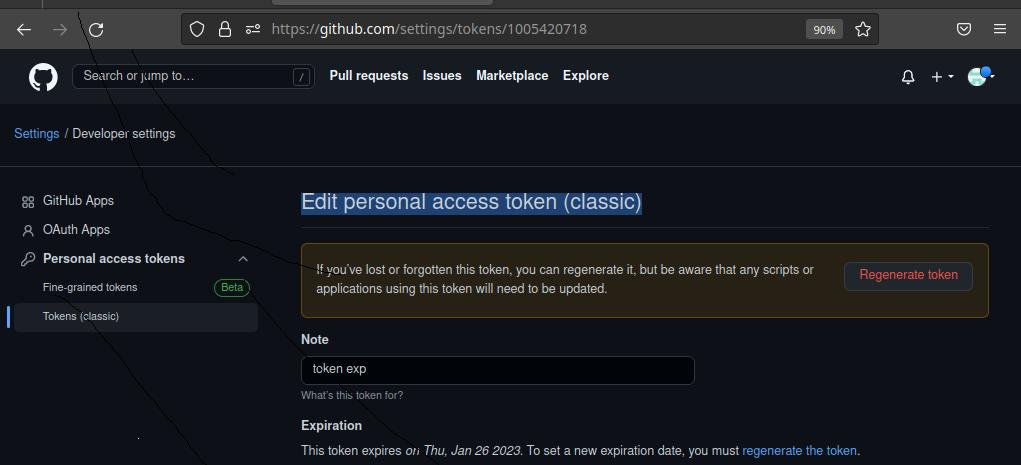
\includegraphics[scale=0.7]{images/c4_1.jpg}
	\caption{Personal Access Tokens}
\end{figure}
\begin{figure}[H] % Ambiente 'figure'
	\centering % imagen sin escalar
	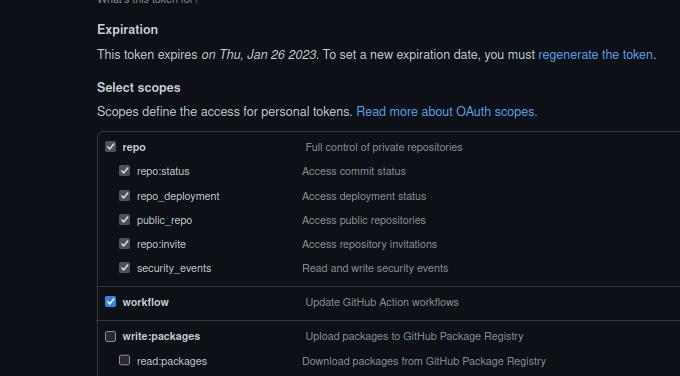
\includegraphics[scale=0.7]{images/c4_2.jpg}
	\caption{Personal Access Tokens}
\end{figure}
\begin{figure}[H] % Ambiente 'figure'
	\centering % imagen sin escalar
	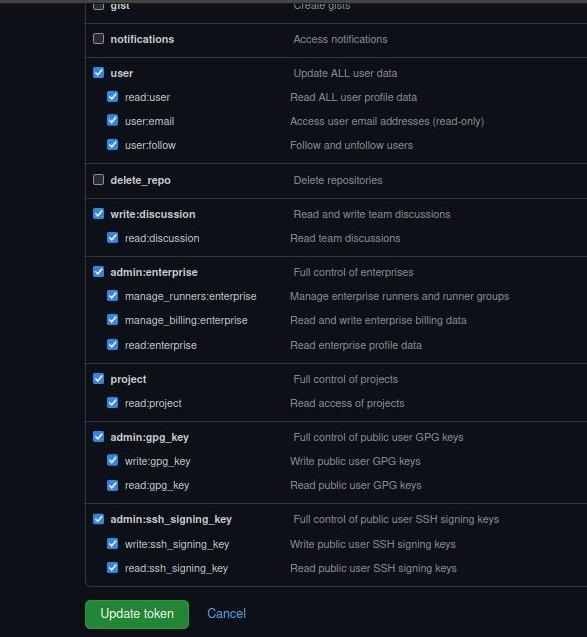
\includegraphics[scale=0.7]{images/c4_3.jpg}
	\caption{Personal Access Tokens}
\end{figure}
Ejecutamos para setear el repositorio.\\
\texttt{git remote set-url origin https://github.com/jdcasasmoviles/nodeapp.git}\\
\section{Git Credential Manager.}
Ahora vamos a instalar y configurar gh.\\
\texttt{type -p curl >/dev/null || sudo apt install curl -y}\\
\texttt{
curl -fsSL https://cli.github.com/packages/githubcli-archive-keyring.gpg | sudo dd of=/usr/share/keyrings/githubcli-archive-keyring.gpg \
\&\& sudo chmod go+r /usr/share/keyrings/githubcli-archive-keyring.gpg \textbackslash{}
\&\& echo "deb [arch=\$(dpkg --print-architecture) signed-by=/usr/share/keyrings/githubcli-archive-keyring.gpg] https://cli.github.com/packages stable main" | sudo tee /etc/apt/sources.list.d/github-cli.list > /dev/null \
\&\& sudo apt update \
\&\& sudo apt install gh -y
}

Luego ejecutamos.\\
\texttt{sudo apt install gh}\\
Verificamos con gh version.\\
\begin{figure}[H] % Ambiente 'figure'
	\centering % imagen sin escalar
	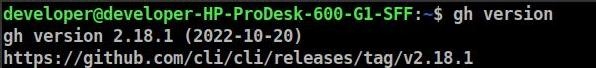
\includegraphics[scale=0.7]{images/c4_4.jpg}
	\caption{gh version.}
\end{figure}
Vamos a configurar con este comando.\\
\texttt{gh auth login}\\

Elegimos las opciones que estan resaltadas en celeste ,como se muestra en la imagen.Finalmente pegamos el token que generamos en nuestra cuenta.\\
\begin{figure}[H] % Ambiente 'figure'
	\centering % imagen sin escalar
	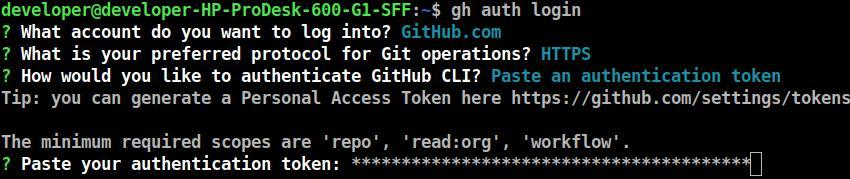
\includegraphics[scale=0.7]{images/c4_5.jpg}
	\caption{gh auth login}
\end{figure}

Enviamos fuentes desde nuestro equipo personal, al repositorio remoto.\\
\texttt{git status}\\
\texttt{git add -A}\\
\texttt{git commit -m "NewCambio"}\\
\texttt{git push origin main}\\
\begin{figure}[H] % Ambiente 'figure'
	\centering % imagen sin escalar
	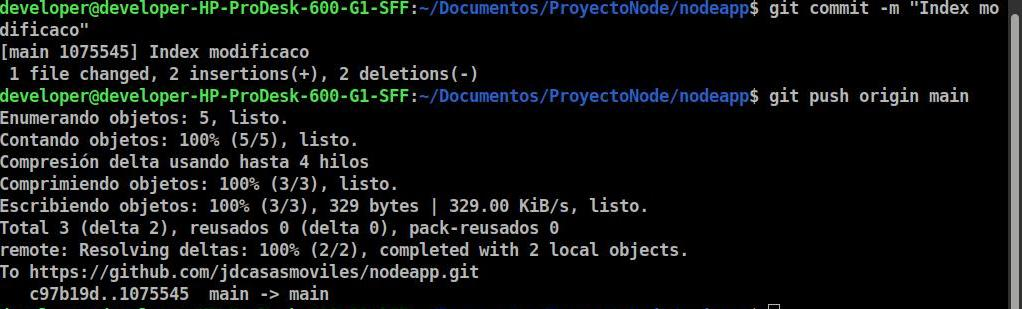
\includegraphics[scale=0.7]{images/c4_6.jpg}
	\caption{Repositorio sincronizando}
\end{figure}

Bajamos el proyecto al servidor en la nube,nos conectamos y ejecutamos.\\
\texttt{ssh userdeploy@35.184.62.239}\\
\texttt{sudo apt-get install git-all}\\
\texttt{git clone https://github.com/jdcasasmoviles/nodeapp.git}\\
Vamos al directorio nodeapp y ejecutamos.\\
\texttt{npm install}\\
Recomendacion es mejor poner el app en el directorio /var/www.\\
\texttt{node server.js}\\
Tenemos que agregar en el servidor cloud una regla para abrir el puerto 3000.En google cloud
 se hace en reglas de firewall en el menu de VM.( si se apaga la maquina el ip cambia).\\
35.184.62.239:3000\\
\begin{figure}[H] % Ambiente 'figure'
	\centering % imagen sin escalar
	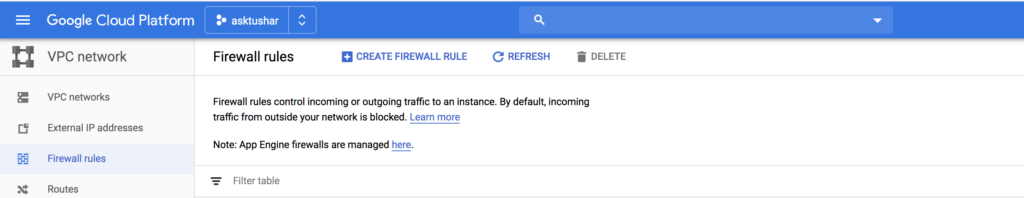
\includegraphics[scale=0.4]{images/c4_7.png}
	\caption{Firewall Rules}
\end{figure}
\begin{figure}[H] % Ambiente 'figure'
	\centering % imagen sin escalar
	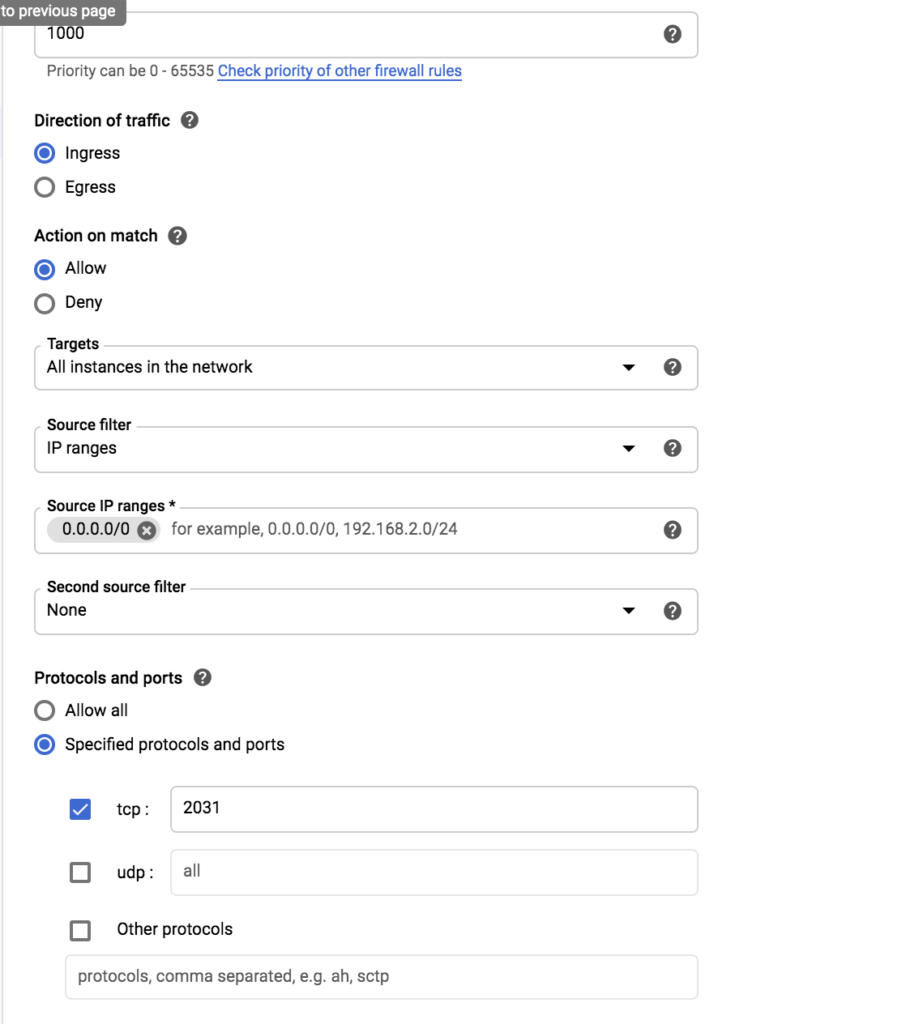
\includegraphics[scale=0.3]{images/c4_8.png}
	\caption{Firewall Rules}
\end{figure}
\begin{figure}[H] % Ambiente 'figure'
	\centering % imagen sin escalar
	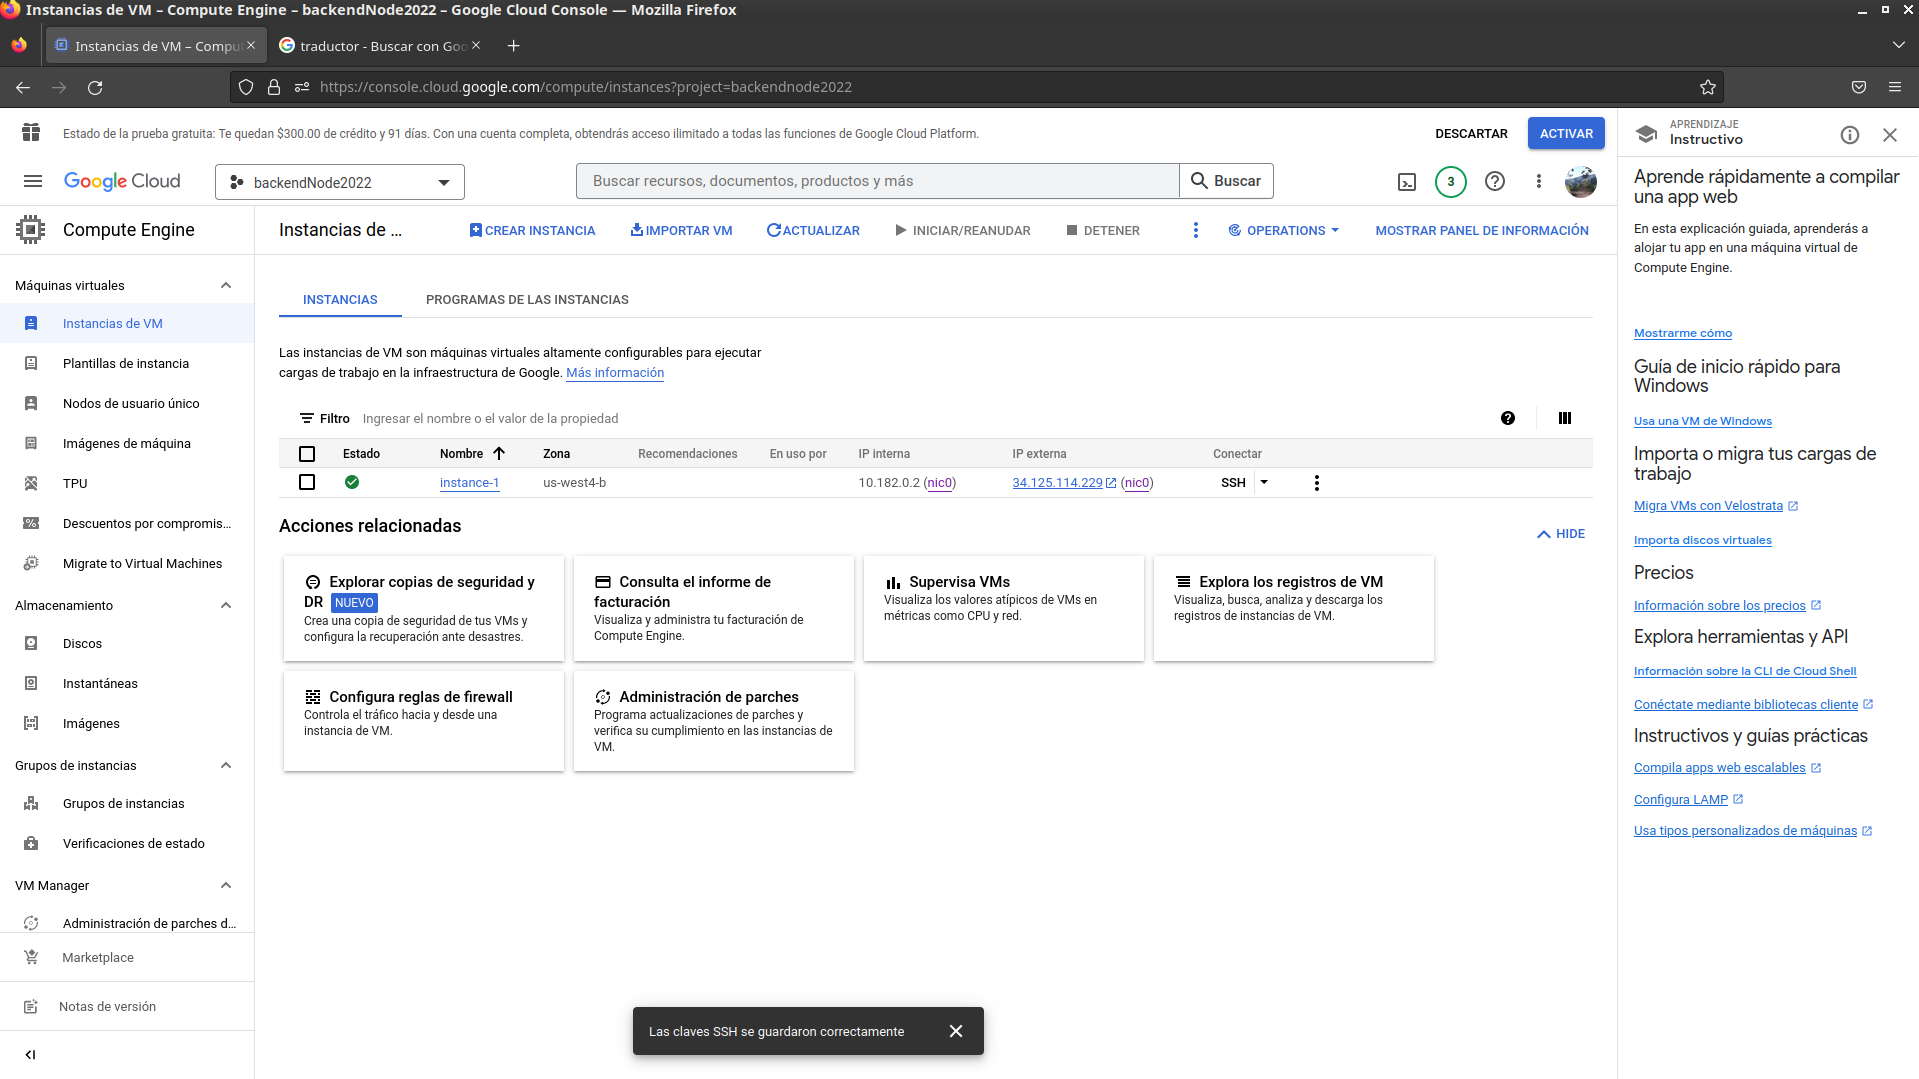
\includegraphics[scale=0.3]{images/c4_9.png}
	\caption{Instancias de VM}
\end{figure}


En el proyecto de node.\\
\texttt{npm install --save-dev nodemon}\\
\texttt{npm install express dotenv}\\
\texttt{const path = require('path');}\\
En el archivo package.json agregar en scripts.\\
\texttt{"start": "NODE\_ENV=production node server",
	"dev": "nodemon server"}\\

\texttt{nodemon server.js}\\

Despliegue en pro.\\
\texttt{npm start}\\
Despliegue en dev.\\
\texttt{npm run dev}\\

Mongo DB.\\
\texttt{sudo apt --fix-broken install ./mongodb-compass\_1.33.1\_amd64.deb}\\